\section{Results}
\label{section:results}

To assess the impact of debloating web applications, we analyze our results
from a number of different perspectives. First, we show the contributions of different application-profiling methods and then compute different metrics
to understand the effectiveness of debloating in terms of reducing the attack-surface of our tested applications. Next, we focus on CVEs to determine whether
debloating can actually remove critical vulnerabilities. Then, we take
a closer look at the bloat introduced by external packages along with the
security implications that come with using this specific development practice.
Finally, we look at what has effectively been removed in debloated applications and test a number of exploits against the original and debloated versions of the evaluated web applications.
% we use clustering to find which parts of the application are more affected by debloating.
  
\begin{figure*}[t]
  \centering
  \begin{subfigure}[b]{0.7\textwidth}
      
\includegraphics[width=\textwidth]{figures/lim/venn_legend.pdf}
      \vspace{-5ex}
  \end{subfigure}

    \begin{subfigure}[b]{0.24\textwidth}
        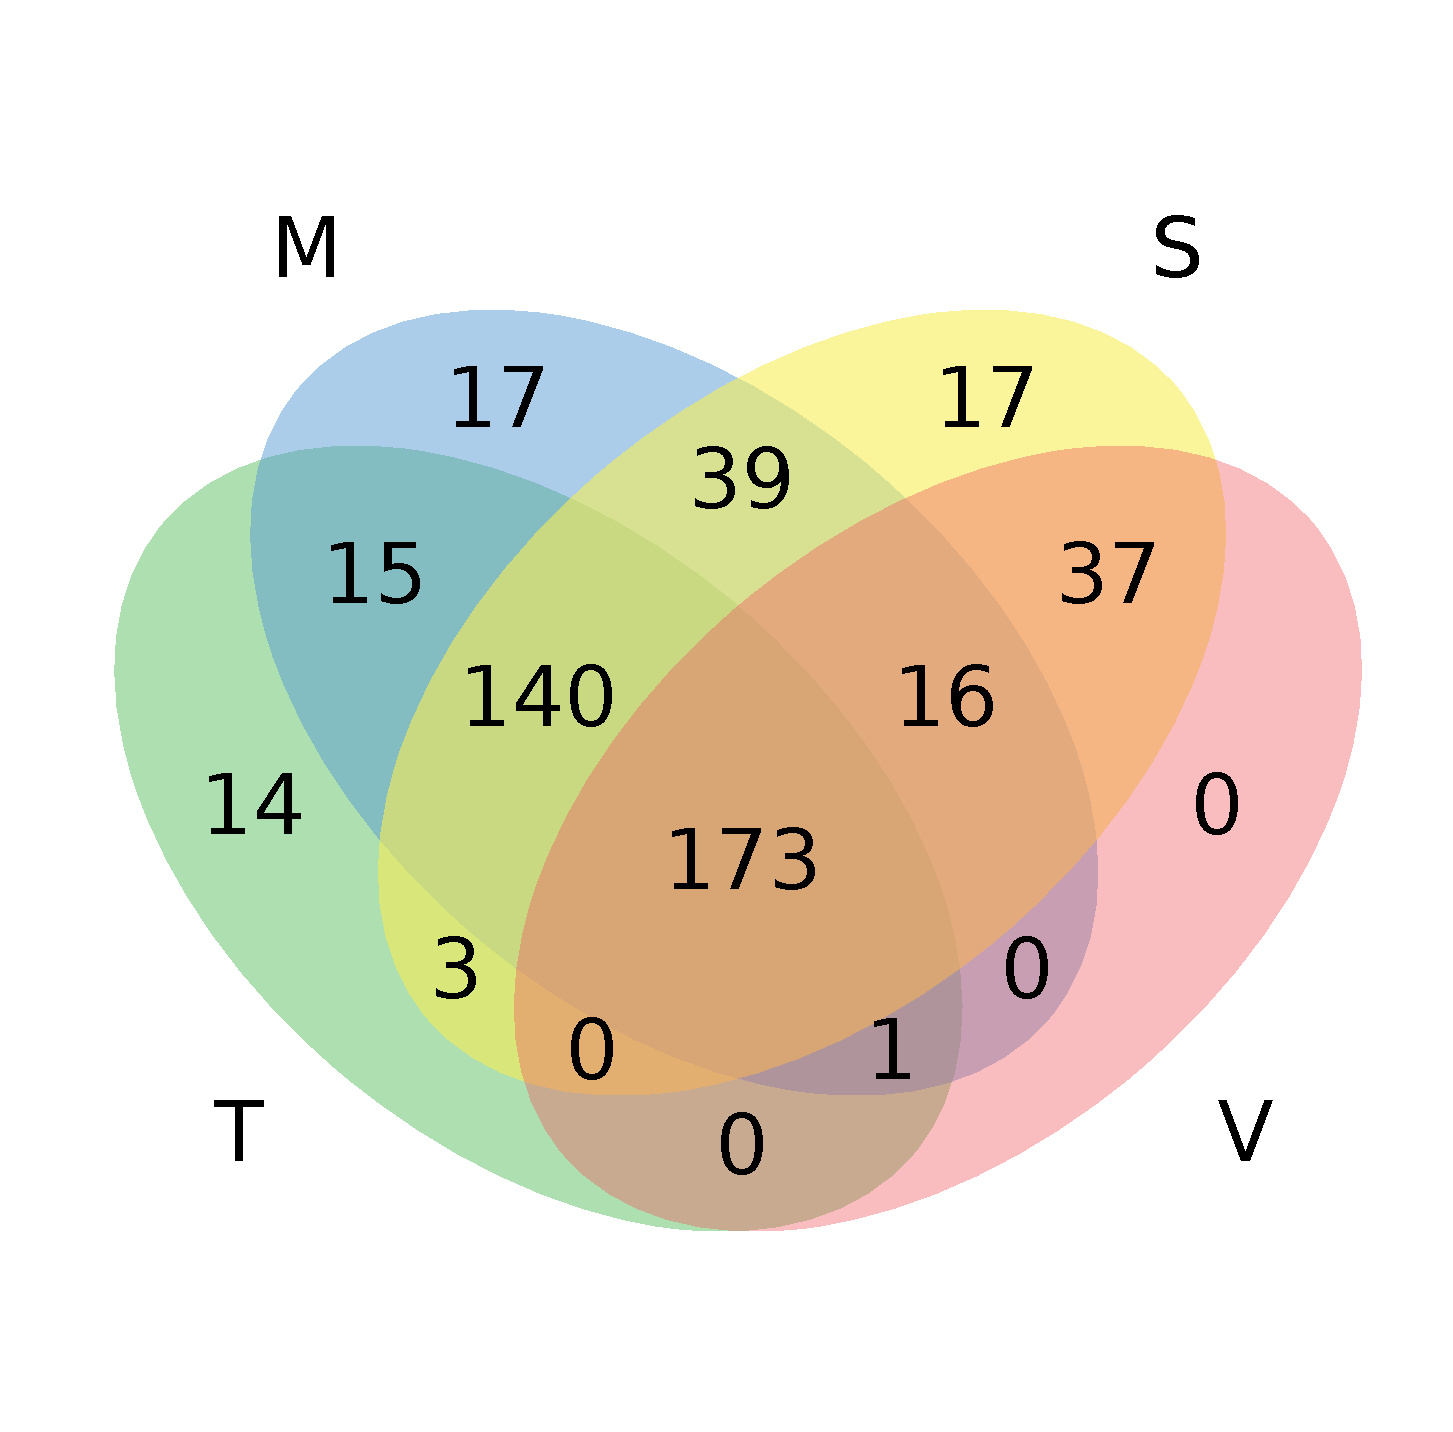
\includegraphics[width=\textwidth]{figures/lim/venn_pma.pdf}
        \caption{\scriptsize phpMyAdmin 4.7.0}
        \label{fig:venn_pma}
    \end{subfigure}
    \begin{subfigure}[b]{0.24\textwidth}
          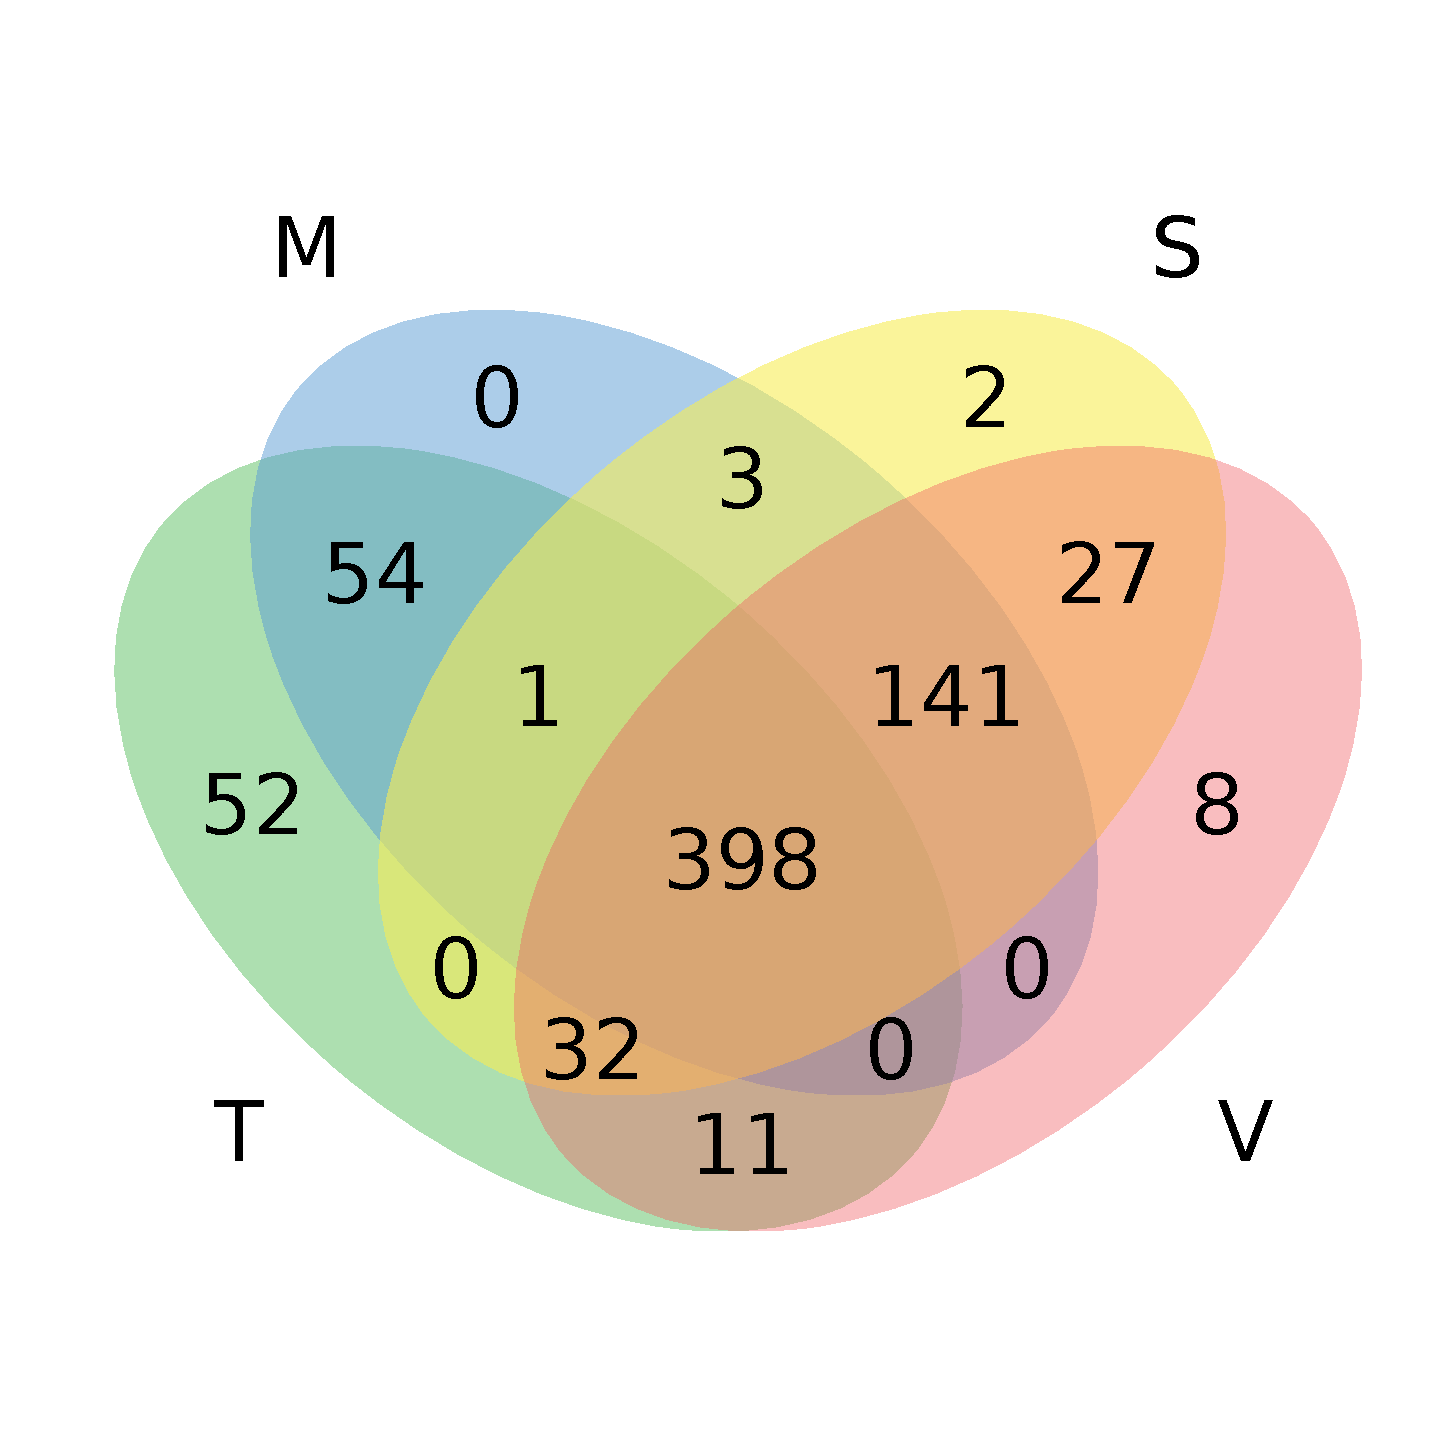
\includegraphics[width=\textwidth]{figures/lim/venn_mwk.pdf}
          \caption{\scriptsize MediaWiki 1.28.0}
          \label{fig:venn_mwk}
    \end{subfigure}
    \begin{subfigure}[b]{0.24\textwidth}
          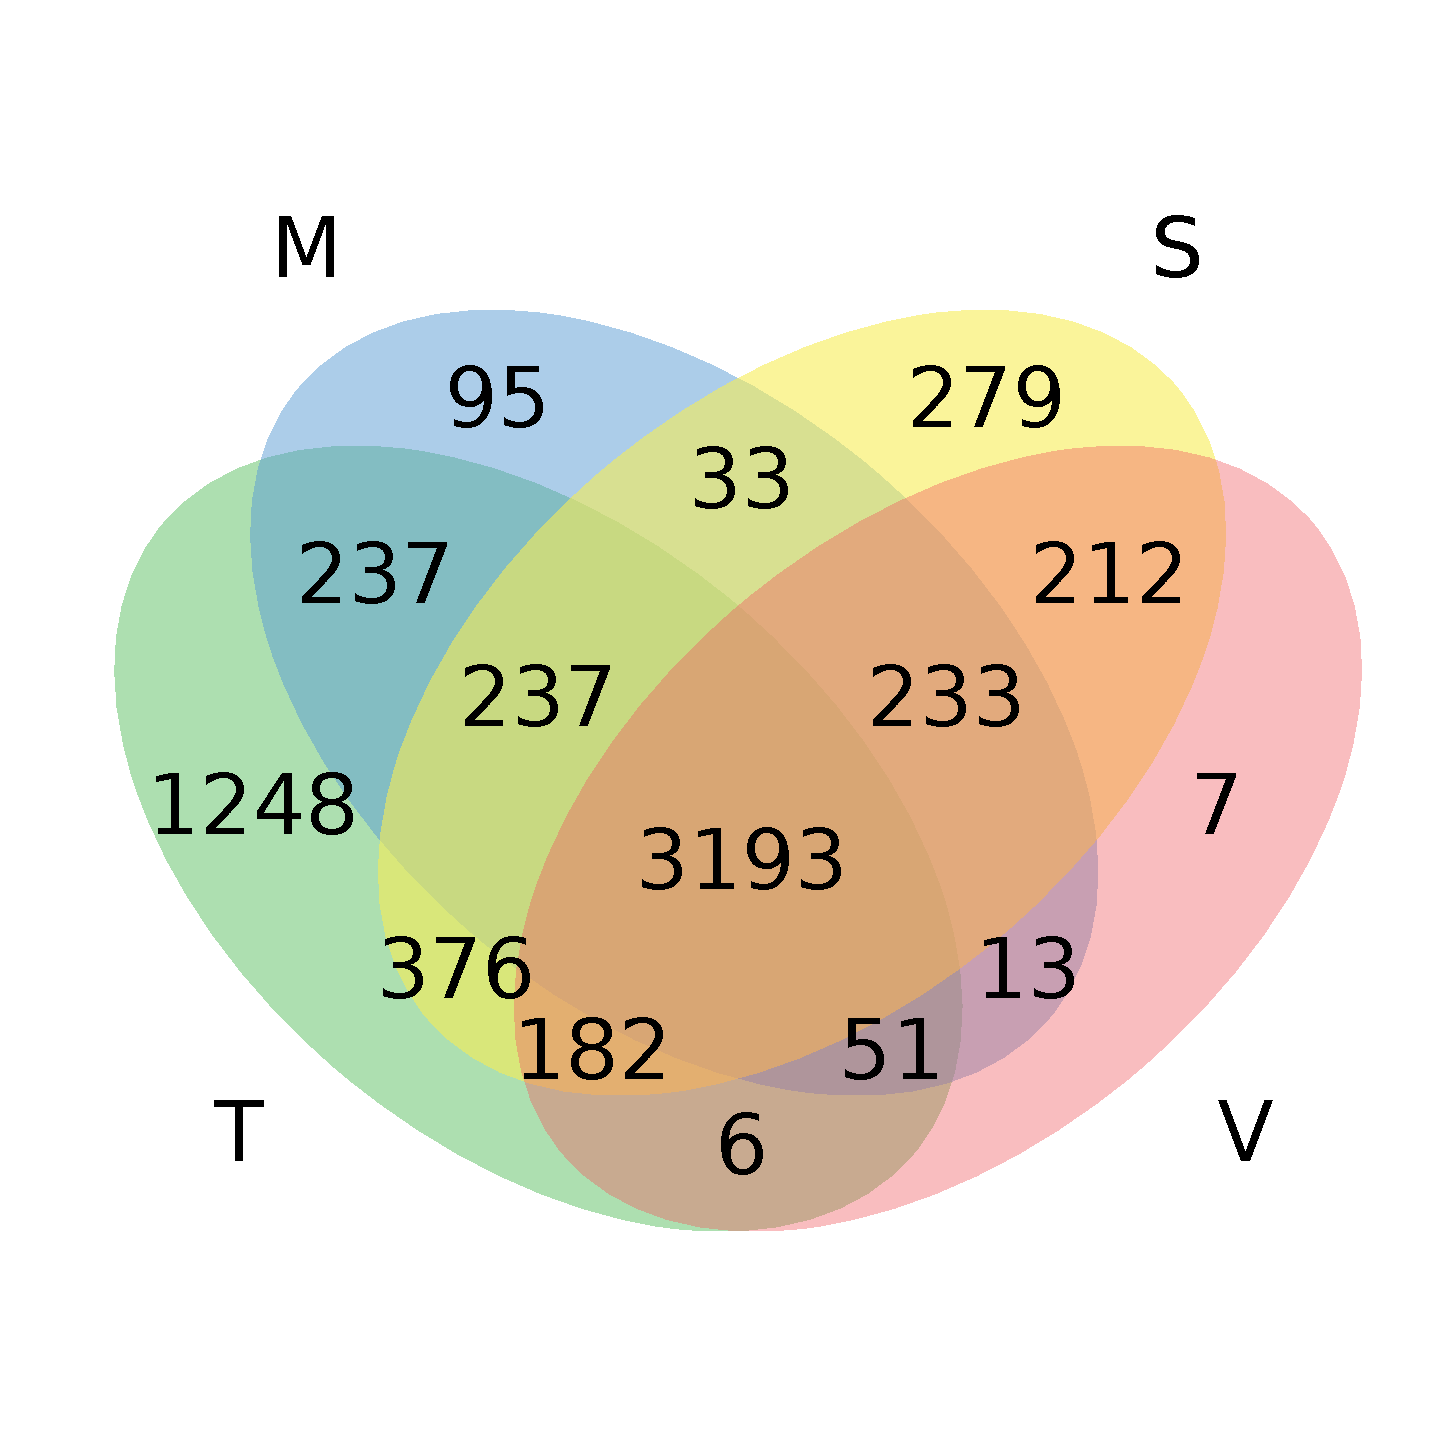
\includegraphics[width=\textwidth]{figures/lim/venn_mgt.pdf}
          \caption{\scriptsize Magento 2.0.5}
          \label{fig:venn_mgt}
    \end{subfigure}
    \begin{subfigure}[b]{0.24\textwidth}
          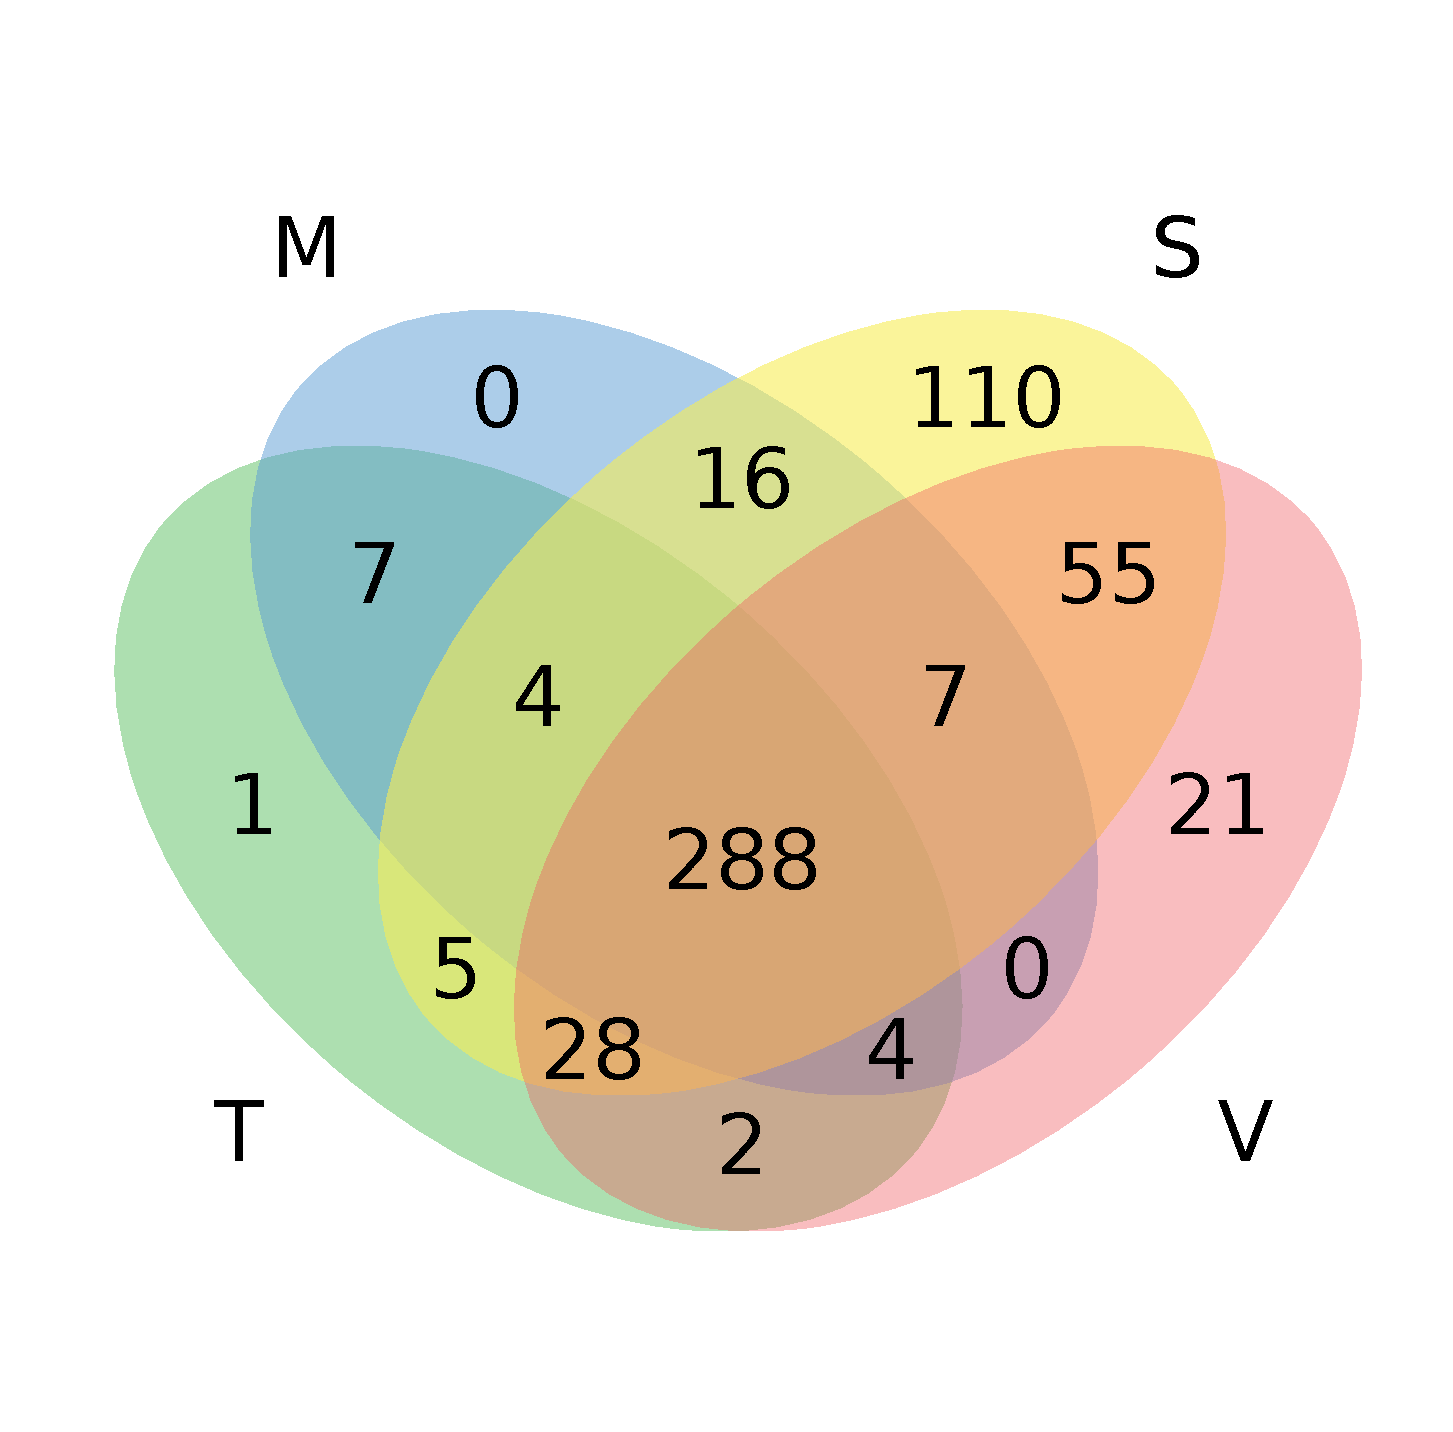
\includegraphics[width=\textwidth]{figures/lim/venn_wp.pdf}
          \caption{\scriptsize WordPress 4.7.1}
          \label{fig:venn_wp}
    \end{subfigure}
  \caption{Venn Diagrams showing covered files during the execution of Tutorials, Crawler, Monkey testing and Vulnerability scanner}
  \label{fig:venncoverage}
\end{figure*}

%Property Oriented Programing (POP) is an exploitation technique in PHP which works similar to ROP (Return Oriented %Programming) and is used to exploit POI vulnerabilities. In this technique, the attacker creates exploit gadgets from %available code in the applications. Each object within the chain performs malicious actions or prepares the environment for %execution of next object in the chain upon deserialization. Dahse et al. have studied automatic generation of such gadget %chains in \cite{Dahse:2014:CRA:2660267.2660363}.

\subsection{Tutorials vs. Monkey Testing vs. \\Crawling vs. Vulnerability Scanning}
As described in Section~\ref{subsec:profiling}, to ensure that we exercise web applications in an objective and repeatable way, we utilized tutorials, monkey testing, crawlers, and vulnerability scanners. Figure~\ref{fig:venncoverage} shows the coverage, in terms of server-side files, that each method obtained on the latest version of each web application in our testbed. We can clearly see that all four methods are required, with each method contributing differently for different web applications.
For example, tutorials trigger more files in Magento compared to other applications, while Spider covers most unique files in WordPress.

%For example, while monkey testing appears to be responsible for triggering the vast majority of source code in MediaWiki, it does not perform nearly as well for the %remaining two applications.

\subsection{Debloating by the numbers}
To evaluate the effectiveness of our two debloating strategies, we computed different metrics that provide
insights into what has actually been removed during the debloating process.


\subsubsection{Logical lines of code}
\label{subsubsec:lloc}
The size of a program positively correlates with the number of programming errors (i.e., bugs). According to McConnel~\cite{mcconnell2004code}, the industry average, at least in 2004, was to have between 1 and 25 bugs for every one thousand lines of code. Given the importance of the size of an application to its overall security, we start by estimating the reduction of the attack-surface by looking at the
Logical Lines Of Code (LLOC, sometimes also called Effective Lines Of
Code). LLOC is intended to measure lines of code without comments, empty
lines and syntactic structure required by the programming language. LLOC
reduction is a robust and precise indicator of how much the volume of
the code was reduced.
Figure~\ref{fig:lloc} reports on the LLOC for all versions of the applications
we debloated.

\paragraph{Number of logical lines over time.}
Looking at the number of LLOC of the original applications, we can observe two different evolution behaviors.
For WordPress, the amount of code is stable and there is even a small decrease of 2\% of LLOC between versions 4.7 and 4.7.1.
For the other applications, we observe the opposite where the source code in the latest versions spikes, compared to the ones released just before them: 82\% LLOC increase for phpMyAdmin, 99\% for MediaWiki, and 171\% for Magento. By
analyzing the code of these newer versions in an attempt to understand their
sudden expansion in size, we discovered that these spikes can be attributed to
a change in development practices, namely the reliance on external packages.
As WordPress does not rely on external packages, it does not exhibit this kind of behavior. We
discuss the issue of relying on external packages in more detail in Section~\ref{subsec:external}.


\begin{figure}[t]
  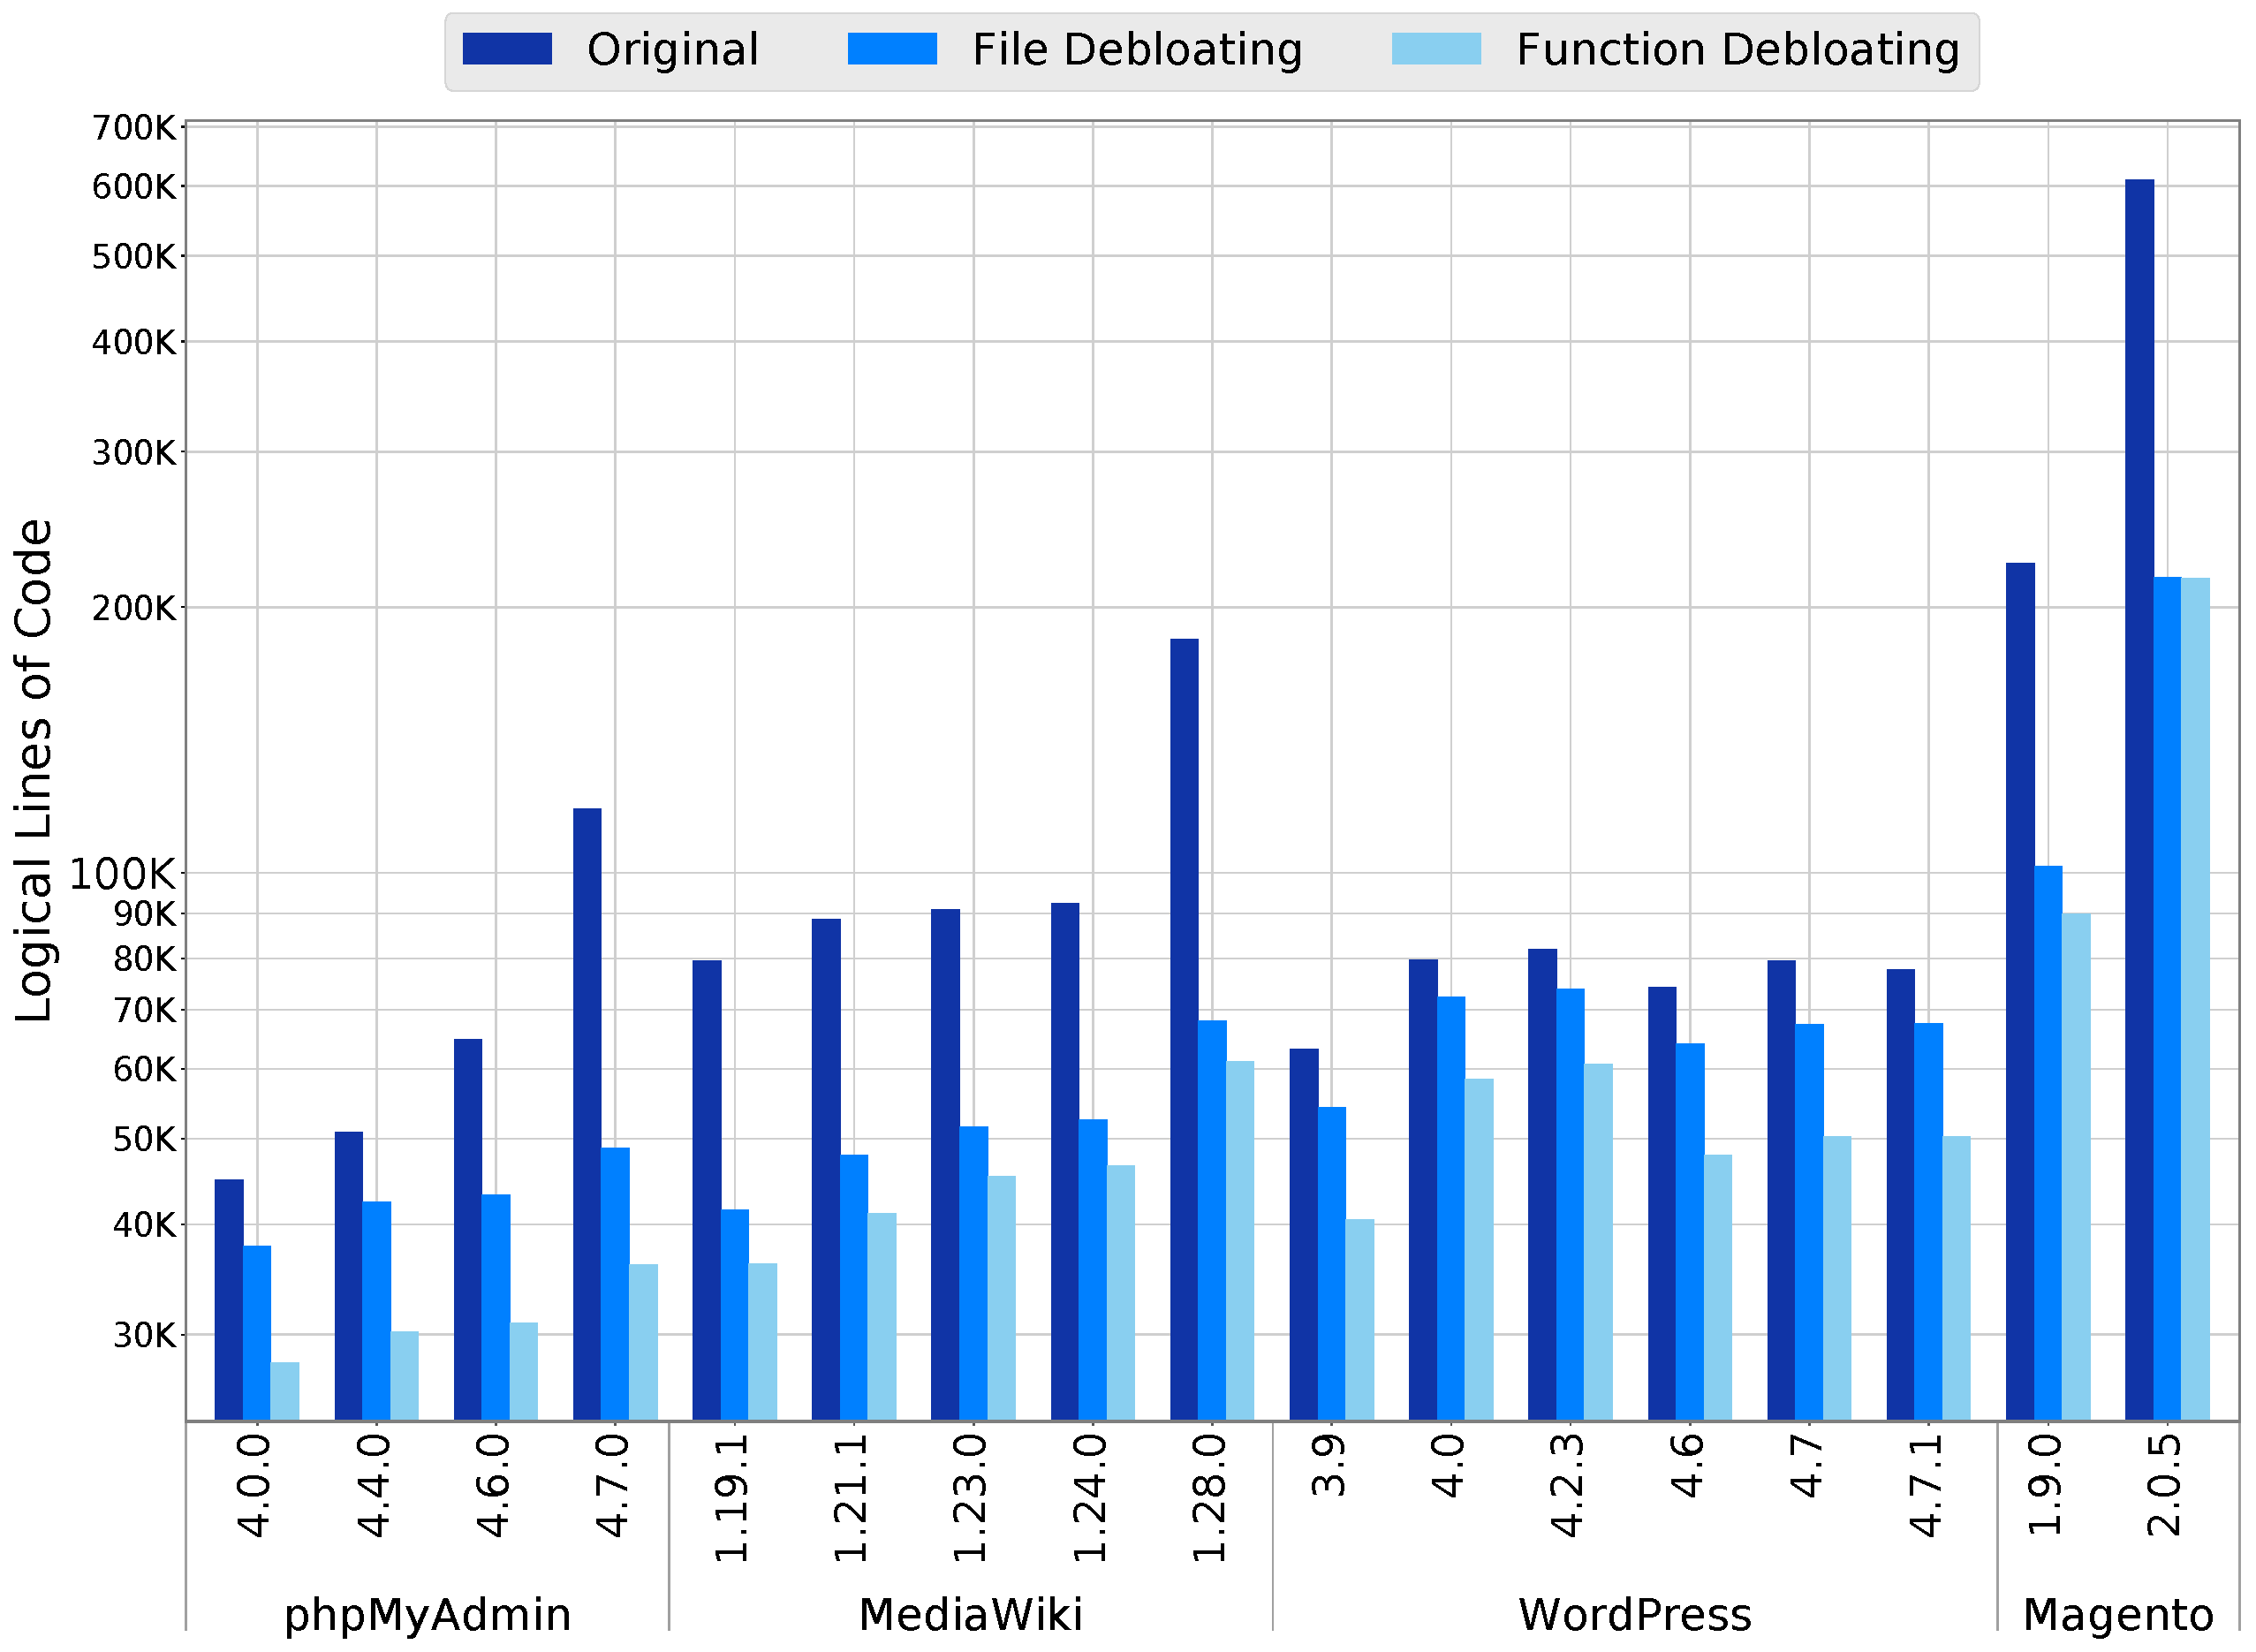
\includegraphics[width=\linewidth]{figures/lim/lloc.pdf}
  \caption{Logical Lines of Code before and after debloating}
  \label{fig:lloc}
\end{figure}


\paragraph{File-level debloating.}
Overall, file-level debloating, the most conservative of the two evaluated
debloating strategies, is already effective in reducing the number of LLOC with an average of 33.1\% reduction.
The minimum observed in our experiment is 9.2\% for WordPress
v.4.0 and a maximum of 64.5\% for Magento v.2.0.5. For Magento,
this reduction represents a removal of 393K lines of code.
This number is a clear sign that large web applications encompass many
different features that may not be used by all users and therefore result
in bloated applications with an unnecessarily large attack-surface. At the same time, it is worthwhile repeating that all debloating results presented in this section are conditional to how web applications are used. Therefore, these large levels of debloating cannot be guaranteed for all possible deployments of web applications. We discuss this issue in Section~\ref{sec:limitations}.

\paragraph{Function-level debloating.}
On average, function-level debloating is able to remove 46.8\% of lines of code.
For both Magento and MediaWiki, it can remove up to
7\% more code over file-level debloating. For phpMyAdmin and WordPress, we observe an
increase of debloating capability of up to 24\%. This
larger reduction (compared to MediaWiki and Magento) is mainly due to
the differences in software development practices.

Compared to the other
tested applications, phpMyAdmin and WordPress are more monolithic with a smaller number of large
source-code files. Since file-level debloating only removes files when none
of their functions were executed, the monolithic nature of these two applications resists
this kind of coarse-level debloating. Contrastingly, Magento and MediaWiki
are developed in a much more modular fashion (many small files each responsible
for a small number of well-defined tasks) and therefore lend themselves better to file-level
debloating. The more fine-grained, function-level debloating bypasses this
issue and can therefore reduce the attack-surface of a web application,
even for more monolithic web applications.


\subsubsection{Cyclomatic complexity}
\label{subsubsec:cyclomatic-complexity}
Next, we look at the evolution of cyclomatic complexity (CC). CC is defined as
the number of linearly independent paths through the code of
an application~\cite{mccabe1976complexity}. A high CC for a
single class implies complicated code that is difficult to
debug and maintain~\cite{gill1991cyclomatic} and therefore
more prone to contain vulnerabilities when compared to code with low
CC~\cite{shin2008empirical,kurmus2013attack}.

\begin{figure}[t]
  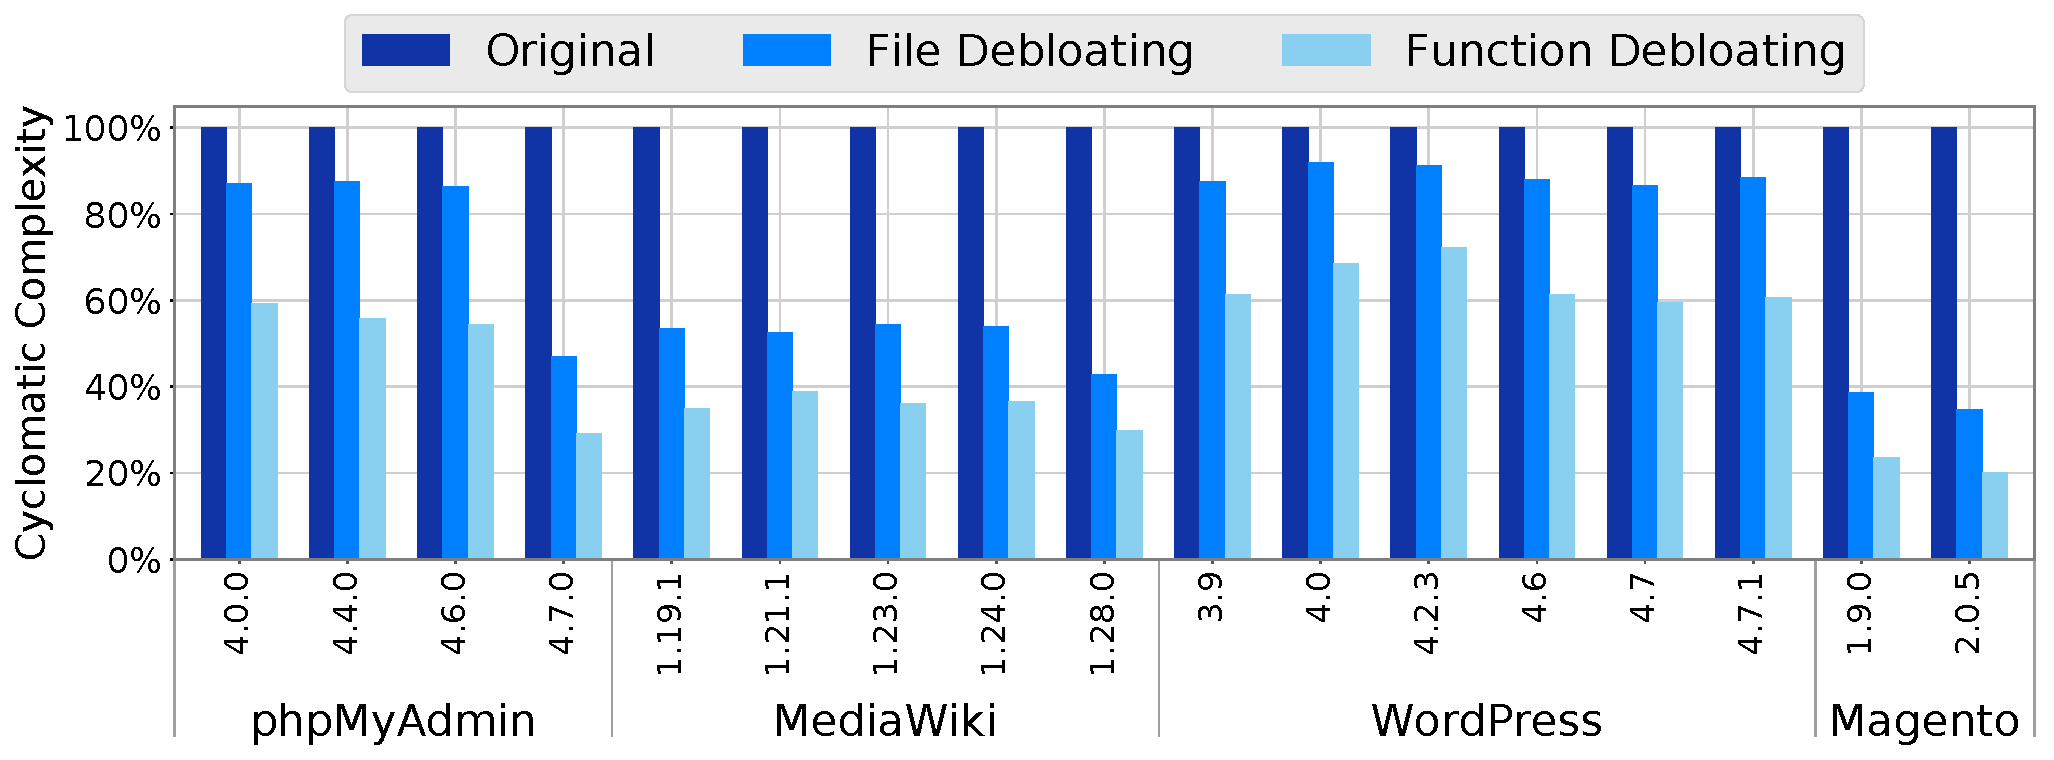
\includegraphics[width=\linewidth]{figures/lim/cc_over_loc.pdf}
  \caption{Evolution of cyclomatic complexity before and after debloating}
  \label{fig:ccoverloc}
\end{figure}

Figure~\ref{fig:ccoverloc} reports on the evolution of the overall CC for
each tested version in our experiment. File-level debloating decreases
CC between 5.9\% to 74.3\% with an average of 32.5\%.
Function-level debloating decreases the program complexity between 23.8\% and 80.2\% with an average of 50.3\%.
These statistics demonstrate that
debloating can remove complex instructions and execution paths in addition to
simple ones. Moreover, the difference between file-level and function-level
debloating shows that code removal through function-level debloating is much
more suited to all kinds of web applications as shown earlier through LLOC
reduction achieved via function-level debloating.


\subsection{Analysis of CVEs}
In this section, we investigate the number of removed CVEs after debloating
along with the effects of debloating on different vulnerability categories.

\subsubsection{CVE reduction after debloating}
\label{sec:cve_reduction}
One practical way to measure the security benefits of debloating web
applications is to study the effects of debloating on known historical
vulnerabilities. If vulnerabilities were part of the core functionality of the
program, the evaluated debloating strategies will not be able to remove the
code associated with them. However, if some vulnerabilities reside in parts
of a web application that are not commonly used, the process of debloating
can effectively remove them.

\begin{table}[t]
  \caption{Number of CVEs removed after application debloating}
  \centering
  \adjustbox{max width=\linewidth}{
  \begin{tabular}{|c|l|l|l|l|l|}
  \hline
  \multicolumn{1}{|l|}{\textbf{Application}} & \textbf{Strategy}   & \multicolumn{2}{l|}{\begin{tabular}[c]{@{}l@{}}\textbf{Total}\\ \textbf{Removed CVEs}\end{tabular}} & \multicolumn{2}{l|}{\begin{tabular}[c]{@{}l@{}}\textbf{Removed}\\ \textbf{Exploitable CVEs}\end{tabular}} \\ \hline
  \multirow{2}{*}{phpMyAdmin}       & File Debloating     & 4/20                                    & 20 \%                                   & 3/19                                      & 15.7 \%                                     \\ \cline{2-6}
                                    & Function Debloating & 12/20                                   & 60 \%                                   & 11/19                                     & 57.8 \%                                     \\ \hline
  \multirow{2}{*}{MediaWiki}        & File Debloating     & 8/21                                    & 38 \%                                   & 3/16                                      & 18.7 \%                                     \\ \cline{2-6}
                                    & Function Debloating & 10/21                                   & 47.6 \%                                 & 5/16                                      & 31.2 \%                                     \\ \hline
  \multirow{2}{*}{WordPress}        & File Debloating     & 0/20                                    & 0 \%                                    & 0/20                                      & 0 \%                                        \\ \cline{2-6}
                                    & Function Debloating & 2/20                                    & 10 \%                                   & 2/20                                      & 10 \%                                       \\ \hline
  \multirow{2}{*}{Magento}          & File Debloating     & 1/8                                     & 12.5 \%                                 & 1/8                                       & 12.5 \%                                     \\ \cline{2-6}
                                    & Function Debloating & 3/8                                     & 37.5 \%                                 & 3/8                                       & 37.5 \%                                     \\ \hline
  \end{tabular}
  }
  \label{table:debloatingcvesresults}
  \end{table}

Table~\ref{table:debloatingcvesresults} compares the effectiveness of
debloating strategies by listing the fractions of removed CVEs. We consider
a vulnerability to have been successfully removed if all the lines of code
and functions associated with that vulnerability were removed during the
stage of debloating. This is a conservative approach as one modification
performed on a single line could thwart a complete attack. As such, the
numbers we report in this section can be interpreted as lower bounds of
the actual number of removed CVEs.


In terms of configuration, we selected the default one for each application.
However, certain vulnerabilities may not be exploitable under this configuration.
For example, there exists 5 CVEs in our dataset for MediaWiki which require file upload functionality to be enabled. Since this option is disabled by default, we make an explicit distinction in the table.
``Total Removed CVEs'' is the total number of CVEs removed by debloating regardless of whether the vulnerable code is enabled or disabled through a configuration option. ``Removed Exploitable CVEs'' reports on the CVEs that are reachable under default configurations of target web applications.
%Certain vulnerabilities may not be exploited under the default configuration of target applications. For example there exists 5 CVEs in our dataset for MediaWiki which require file upload functionality to be enabled. Since this option is disabled by default,
%we ran our tests with and without this feature enabled and reported both numbers.
%``Total Removed CVEs`` is the the total number of CVEs removed by debloating regardless of vulnerable code being enabled through configuration settings and ``Removed Exploitable CVEs'' reports on the CVEs that are reachable under default configurations of target web applications.

On average, we discovered that up to 38~\% of vulnerabilities are removed by
file debloating whereas 10-60~\% are removed by function debloating. As
shown in Table~\ref{table:debloatingcvesresults}, function-level debloating
can triple (in the case of phpMyAdmin and Magento) the number of removed CVEs, compared to file-level debloating. This
behavior can be generalized to web applications that do not have CVE
information and demonstrates that the reduction of a web application's
LLOC (Section~\ref{subsubsec:lloc}) and its cyclomatic complexity
(Section~\ref{subsubsec:cyclomatic-complexity}) translates to a reduction
of concrete vulnerabilities. Wordpress is a clear negative outlier with only
10\% CVE reduction, even through the more flexible function-debloating
strategy. As mentioned earlier, WordPress is a relatively monolithic
application and most of our mapped CVEs are located in core WordPress code (e.g.,
Authentication, CSRF tokens, and post/comment-related actions) which cannot
be removed by our debloating framework.








\begin{figure}[t]
  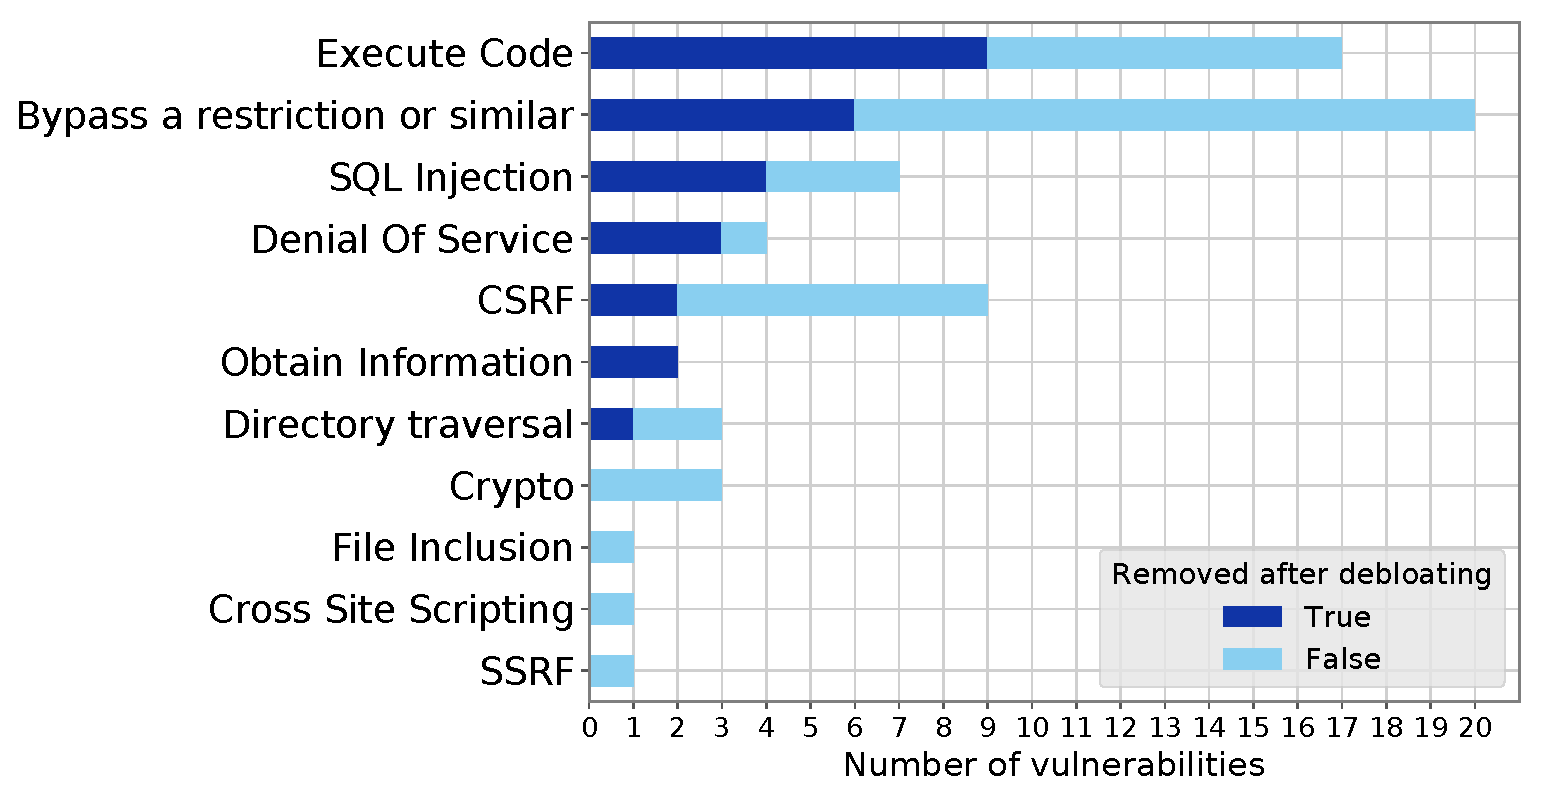
\includegraphics[width=\linewidth]{figures/lim/vuln_per_category.pdf}
  \caption{Vulnerability Categories}
  \label{fig:vulnpercat}
\end{figure}

\subsubsection{Types of CVEs in analyzed web applications}

Even though our results demonstrate the ability to remove vulnerabilities
from web applications through the use of debloating, one may wonder
whether debloating is better suited for some types of vulnerabilities over
others. Figure~\ref{fig:vulnpercat} provides details on the categories of
the CVEs we removed through debloating.


One can observe that for certain classes of vulnerabilities, such as,
Denial-of-Service attacks and Information-Revealing vulnerabilities,
debloating can almost completely remove them.
For others, such as, restriction bypassing, command execution, and
SQL injection, debloating can substantially reduce them.
Our interpretation of these findings has to do with the maturity of
the evaluated web applications. Specifically, all four web applications
have been available for a long period of time, allowing many shallow
vulnerabilities to have already been discovered and corrected. The remaining
vulnerabilities are likely to be situated in parts of a web application that
are less commonly exercised. For example, the code-execution vulnerabilities
that can be removed for phpMyAdmin are inside very specific features, such as,
the ability to export PHP arrays (CVE-2016-6609), the support of the
ZIP extension while importing data (CVE-2016-6633), and the abilities
to copy table definitions (CVE-2013-3238) and perform Regex search and replace over table columns
(CVE-2016-5734).


Contrastingly, the three cryptography-related vulnerabilities we analyzed are
still present in the debloated versions of web applications. One of the CVEs
related to this category is about a flaw in the cookie encryption algorithm in
phpMyAdmin (CVE-2016-6606). Since every page interacts with user
cookies to, at the very least, verify them, vulnerable code cannot be
removed. Another vulnerability in this category relates to an insecure random
number generator used in cryptographic operations by Magento (CVE-2016-6485).
This vulnerability exists in a constructor of the main encryption
classes which is widely used throughout the application. When considered
together, these findings suggest that cryptography-related vulnerabilities
are a core part of web applications and thus unlikely to be removed through
the process of debloating.


\subsection{External packages}
\label{subsec:external}

% \begin{table*}[t]
%   \caption{Statistics on the external packages included in web applications and the effects of debloating in terms of reducing their LLOC.}
%   \centering
%   \adjustbox{max width=\linewidth}{
%   \begin{tabular}{c|c|c|c|c|c|c|}
%   \cline{2-7}
%    & \multicolumn{3}{c|}{\textbf{Before debloating}} & \multicolumn{3}{c|}{\textbf{After function-level debloating}} \\ \hline
%   \multicolumn{1}{|c|}{\multirow{2}{*}{\textbf{Application}}} & \multirow{2}{*}{\begin{tabular}[c]{@{}c@{}}\# \textit{lines in main}\\\textit{application}\end{tabular}} & \multirow{2}{*}{\begin{tabular}[c]{@{}c@{}}\textit{\# lines in}\\\textit{packages}\end{tabular}} & \multirow{2}{*}{\textit{\# packages}} & \multirow{2}{*}{\begin{tabular}[c]{@{}c@{}}\textit{\# lines in main}\\ \textit{application}\end{tabular}} & \multirow{2}{*}{\begin{tabular}[c]{@{}c@{}}\textit{\# lines in}\\\textit{packages}\end{tabular}} & \multirow{2}{*}{\begin{tabular}[c]{@{}c@{}}\textit{\# packages}\\\textit{completely removed}\end{tabular}} \\
%   \multicolumn{1}{|c|}{} &  &  &  &  &  & \\ \hline
%   \multicolumn{1}{|c|}{phpMyAdmin 4.7.0} & 35,739  & 82,604  & 45 & 26,377 (-26.2\%)  & 9,653 (-88.3\%)  & 38 (84.4\%)  \\ \hline
%   \multicolumn{1}{|c|}{MediaWiki 1.28.0}   & 133,019 & 50,898  & 40 & 54,827 (-58.8\%)  & 6,285 (-87.7\%)  & 24 (60.0\%)  \\ \hline
%   \multicolumn{1}{|c|}{Magento 2.0.5}      & 396,448 & 212,906 & 71 & 181,696 (-54.2\%) & 34,038 (-84.0\%) & 58 (81.7\%)  \\ \hline
%   \end{tabular}
%   }
% \label{table:numberofpackages}
% \end{table*}

\begin{table*}[t]
  \caption{Percentage of removed LLOC from external packages.}
  \centering
  \adjustbox{max width=\linewidth}{
  \begin{tabular}{|c|c|c|c|c|c|c|c|c|}
  \cline{1-9}
  \multicolumn{3}{|c|}{\textbf{Before debloating}} & \multicolumn{6}{c|}{\textbf{After function-level debloating}} \\ \hline
  \multirow{2}{*}{\begin{tabular}[c]{@{}c@{}}\# \textit{lines in main}\\\textit{application}\end{tabular}} & \multirow{2}{*}{\begin{tabular}[c]{@{}c@{}}\textit{\# lines in}\\\textit{packages}\end{tabular}} & \multirow{2}{*}{\textit{\# packages}} & \multirow{2}{*}{\begin{tabular}[c]{@{}c@{}}\textit{\# lines in main}\\ \textit{application}\end{tabular}} & \multirow{2}{*}{\begin{tabular}[c]{@{}c@{}}\textit{\# lines in}\\\textit{packages}\end{tabular}} & \multirow{2}{*}{\begin{tabular}[c]{@{}c@{}}\textit{\# packages}\\\textit{completely}\\\textit{removed}\end{tabular}} & \multicolumn{3}{c|}{\begin{tabular}[c]{@{}c@{}}\textit{\# packages where a given \%}\\\textit{lines were removed}\end{tabular}} \\ \cline{7-9}
  \multicolumn{1}{|c|}{}  &  &  &  &  &  & \textgreater{}\textit{70\%} & \begin{tabular}[c]{@{}c@{}}\textless{}\textit{70\% and}\\ \textgreater{}\textit{30\%}\end{tabular} & \textless{}\textit{30\%}\\ \hline
  \multicolumn{9}{|c|}{\textbf{phpMyAdmin 4.7.0}} \\ \hline 
  35,739  & 82,604  & 45 & 26,377 (-26.2\%)  & 9,653 (-88.3\%)  & 38 (84.4\%) & 2 & 1  & 4  \\ \hline
  \multicolumn{9}{|c|}{\textbf{MediaWiki 1.28.0}} \\ \hline 
  133,019 & 50,898  & 40 & 54,827 (-58.8\%)  & 6,285 (-87.7\%)  & 24 (60.0\%) & 2 & 2  & 12 \\ \hline
  \multicolumn{9}{|c|}{\textbf{Magento 2.0.5}} \\ \hline 
  396,448 & 212,906 & 71 & 181,696 (-54.2\%) & 34,038 (-84.0\%) & 58 (81.7\%) & 6 & 5  & 2  \\ \hline
  \end{tabular}
  }
\label{table:numberofpackages}
\end{table*}



\subsubsection{Quantifying the bloat from external packages}

In our test bed, phpMyAdmin v.4.7.0, MediaWiki v.1.28.0 and Magento v.2.0.5 rely
on external dependencies that can be downloaded via Composer (WordPress does not rely on external packages). As described in
Section~\ref{sec:background}, Composer is a package manager for PHP (similar
to the NPM manager for NodeJS applications) which allows web applications
to specify which external packages they rely on and have these packages be
tracked and updated.

As we briefly discussed in Section~\ref{subsubsec:lloc}, the number of LLOC of
these three specific versions dramatically
increases (compared to prior versions) because of this dependency on external
packages. Table~\ref{table:numberofpackages} provides statistics on the
number of packages pulled by these applications and how much bloat they
provide against our usage profiles.


First, one can observe that external packages introduce a large amount of
unused code. For all three debloated applications, more than 84\% of their code
was removed from them. This means that the attack-surface is unnecessarily
large through the dependency on external packages. The number of removed
lines from external packages for Magento is particularly noteworthy with
more than 178,000 lines of code removed. Moreover, the number of packages
that can be completely removed is also quite large: 84\% for phpMyAdmin,
60\% for MediaWiki and 81\% for Magento. This confirms that most packages
are unnecessary for the usage profiles that we recorded. Finally, focusing
exclusively on the lines of code, phpMyAdmin is the only application where
external packages have more lines than the main application. However, after
debloating, this relationship is reversed with the codebase of phpMyAdmin
being three times the size of the introduced external packages.


Despite the advantages of using package managers (e.g., the ability to track
dependencies and update vulnerable libraries without the need to update
the main application), our findings show that these advantages come at a
considerable cost in terms of unnecessarily expanding the attack-surface of
a web application with code that is seldomly executed. As such, developers
must take special care to include the bare minimum of external packages,
knowing the unwanted side-effects that each external package brings.

\subsubsection{Removing POI gadgets}

\paragraph{What are POI gadgets?}
Property Oriented Programing (POP) is an exploitation technique
in PHP which works similarly to Return Oriented Programming
(ROP)~\cite{shacham2007geometry} and is used to exploit PHP Object Injection
(POI) vulnerabilities~\cite{POI}. In this technique, the attacker creates
exploit gadgets from available code in the applications. By chaining
multiple gadgets within the application, an attacker can usually run
arbitrary code, write to arbitrary files, or interact with a database. Dahse
et al. have studied the automatic generation of such gadget chains for PHP
applications~\cite{Dahse:2014:CRA:2660267.2660363}.

\paragraph{PHP unsafe deserialization.}
The PHP language gives developers the ability to serialize arbitrary objects in
order to store them as text, or transfer them over the network. Deserialization
reverses this process, generating PHP objects from serialized data. This
mechanism can be abused by an attacker to load specific classes in the
application and build a gadget chain. Practical examples of this vulnerability
are when \texttt{unserialize} is called on a database field or value of a
field within a cookie that can be manipulated by the users.

Historically, this attack was very difficult to successfully execute. Attackers
could only build gadgets with the classes that were present in the context of
the vulnerable file. They needed insights into how the application was built
in order to know which classes could be abused for gadgets. However, starting
from PHP 5, the \texttt{\_\_autoload()} magic function~\cite{PHPAutoload}
was introduced and unintentionally made exploitation of deserialization
vulnerabilities easier. This new loading feature was beneficial for PHP
developers who did not have to manually include all the files they wanted to
use at the very top of each of their PHP files. It also helped the adoption
of package managers like Composer, as any external dependency could be easily
called from anywhere in the application. The downside of this new function
was that it also allowed attackers to instantiate any PHP class across the
entire application thereby enabling the easier construction of gadget chains.

In order to build a chain, attackers use these so-called ``magic''
functions~\cite{PHPWakeup} that form the basis of their gadget chain. One of
the functions that is widely used in POI exploits is the \textit{destruct}
function. In Section~\ref{subsec:coverage}, we detailed the challenges in
getting complete coverage of destructors in our tested applications. Accurate
coverage of destructors also allows us to precisely analyze the impact of
debloating on gadget creation.




\paragraph{Can debloating remove gadgets from external packages?}

Given the increased footprint of web applications due to their reliance
on package managers and external dependencies, one may wonder about the
possibility of abuse of these packages for the creation of gadgets. To
measure the effect of debloating on Property-Oriented-Programming (POP)
gadgets, we utilized the PHPGGC~\cite{PHPGGC} library. PHPGGC (which stands
for PHP Generic Gadget Chains) contains a list of known gadgets in popular
PHP packages such as Doctrine, Symfony, Laravel, Yii and ZendFramework. When
a vulnerable PHP application includes any of the packages listed in PHPGGC,
the attackers can generate gadget chains to achieve RCE, arbitrary file
writes, and SQL injections.

We analyzed the available gadget chains in PHPGGC and
checked whether any of our tested PHP applications included these
chains. Table~\ref{table:knowngadgets} summarizes the presence of each gadget
and whether debloating removes them or not. WordPress is not included in this table because it does not rely on external packages.
This does not make WordPress immune to POI attacks, but universally known gadget chains in popular external packages can not be used to exploit WordPress.
%Note that while packages such as Symfony are used across our tested web applications, the specific component required to create gadget chains was not pulled by any of tested applications. Such cases are omitted from our results.
For the affected applications, file-level debloating removes 4/6 gadgets while function debloating removes
6/6 available gadget chains. This again demonstrates the power of debloating
which can not only remove some fraction of vulnerabilities but also make
the exploitation of the remaining ones harder by removing the gadgets that
attackers could abuse during a POI attack.


\begin{table}[]
  \centering
  \caption{List of packages with known POP gadget chains}
\scalebox{0.9}{
\begin{tabular}{|l|l|c|c|}
\hline
\multirow{2}{*}{\textbf{Application}}      & \multirow{2}{*}{\textbf{Package}} & \multicolumn{2}{l|}{\begin{tabular}[c]{c@{}c@{}}\textbf{Removed by}\\\textbf{Debloating}\end{tabular}} \\ \cline{3-4}
    &    & \textit{File}     &  \textit{Function}                                     \\ \hline
\multirow{2}{*}{phpMyAdmin 4.7.0} & Doctrine                 & \faCheck                                         & \faCheck                                            \\ \cline{2-4}
                                  & Guzzle                   & \faCheck                                         & \faCheck                                            \\ \hline
MediaWiki 1.28.0                  & Monolog                  & \faCheck                                         & \faCheck                                            \\ \hline
\multirow{3}{*}{Magento 2.0.5}    & Doctrine                 & \faCheck                                         & \faCheck                                            \\ \cline{2-4}
                                  & Monolog                  & \faTimes                                         & \faCheck                                            \\ \cline{2-4}
                                  & Zendframework            & \faTimes                                         & \faCheck                                            \\ \hline
\end{tabular}}
\label{table:knowngadgets}
\end{table}


\subsubsection{Utilizing development packages in production}
During our analysis of external packages, we identified yet another source
of bloat in new versions of web applications. When declaring external
dependencies through Composer, two options are available: ``require'' and
``require-dev''. The first option indicates packages that are mandatory for
the application to run properly. The second lists packages that should only be
used in development environments, such as, packages providing support for unit
testing, performance analysis, and profiling. We discovered that applications
downloaded from official websites often include these development packages. As
such, when these packages are used to deploy web applications in production
mode, they will contain unnecessary development libraries. This does not
only increase the attack-surface by having unnecessary code bloating the
application, but can also lead to exploitation for misconfigured applications.

CVE-2017-9841 presents one example of such a
vulnerability~\cite{phpunitVulnerability}. Specifically, this CVE refers
to an RCE attack in specific versions of the PHPUnit library, which is
a popular unit testing library for PHP. By default, Composer places all
external packages under ``vendor'' directory. If this specific directory
happens to be accessible through a misconfiguration of the server, PHPUnit
files are then accessible and can be exploited to conduct an RCE attack.

The four web applications that we evaluated for this study, present
different behaviors with respect to development packages. WordPress does not rely on external packages downloaded through Composer.
MediaWiki never
included development packages in its releases. phpMyAdmin had them in version
4.7.0 but stopped including them in version 4.8.3 (the latest at the time of
writing). Magento started including them from version 2.0 and still includes
them today. We have reached out to Magento and informed them about this issue.


\subsection{Qualitative analysis of the removed code}
\label{subsec:qualitative}

In the previous sections, we analyzed the effects of debloating on the source code of applications from a software-engineering perspective (i.e., LLOC and Cyclomatic Complexity reduction) as well as from a security standpoint (i.e., number of CVEs and gadgets removed). At the same time, one may wonder what exactly was removed from each application during the process of debloating.



Given that thousands of files were removed, manually analyzing each file does not scale. As such, we turn to NLP techniques that allow us to cluster the removed files together and provide us with hints about the nature of each cluster. Specifically, we use the k-means clustering algorithm based on text vectors extracted from removed file names and file paths. Each file path includes directories that indicate which library or package, the file belongs to. For most modern web applications, this allows for a reasonable separation of files across different application plugins and modules.
To end up with meaningful clusters, we tuned TFIDF vectorizer parameters along with the number of k-means clusters. We used the TFIDF maximum frequency limit to ignore common terms appearing in more than 50\% of the files. Depending on the size and modularity of the application, 10 to 20 clusters yielded the most instructive grouping of files.

Table~\ref{tab:removed_files_categories} shows the categories of the three largest removed clusters from each web application. Across all four applications, we observe the removal of source code related to external packages (e.g., Symfony for phpMyAdmin, Elastica for MediaWiki, and Zendframework1 for Magento), followed by localization/theme files (e.g., twentyfourteen theme for WordPress), and unused database drivers. We provide more application-specific details of removed features in the next paragraphs.

\begin{table}[t]
  \caption{Features and external packages with the most removed files after file debloating (removed features are marked in italic). Entries marked with $\ast$ are packages that are indirectly pulled by other ``require-dev'' packages (not used by core application) for the purpose of test coverage reporting and coding standard enforcement.}
  \label{tab:removed_files_categories}
  \centering
\adjustbox{max width=\linewidth}{
\begin{tabular}{|l|l|}
\hline
\textbf{Applications} & \textbf{Features/Packages with most files removed} \\ \hline
                           & 1) Guzzle~\cite{guzzle}: ``Generating API HTTP response'' *  \\
\textit{phpMyAdmin 4.7.0}  & 2) Symfony~\cite{Symfony}: ``Parsing configuration files'' * \\
                           & 3) PHP\_CodeSniffer~\cite{PHP_CodeSniffer}: ``Enforcing coding standards'' * \\ \hline
                           & 1) \textit{Messages \& Languages} \\
\textit{MediaWiki 1.28.0}  & 2) Less.php~\cite{less.php}: ``Generating CSS code'' \\
		                       & 3) Elastica~\cite{elastica}: ``Elastic search interface used by\\ & extensions'' \\ \hline
                           & 1) Twentyfourteen theme~\cite{twentyfourteen_theme} \\
\textit{WordPress 4.7.1}	 & 2) Twentytwelve theme~\cite{twentytwelve_theme} \\
		                       & 3-4) Also theme related \\
		                       & 5) \textit{Multi-site administration} \\ \hline
	                         & 1) Zendframework1~\cite{zendframework1}: ``Generating web pages and\\
\textit{Magento 2.0.5}     & database operations'' \\
		                       & 2) \textit{Sales, Orders \& Credit Memo} \\
		                       & 3) \textit{Internal framework filters \& Views} \\ \hline
\end{tabular}
}
\end{table}

\vspace{0.5ex}
\noindent\textbf{phpMyAdmin's} removed features include the uploading of plugins, GIS visualizations, and unused file formats used in import/export (such as, Dia, EPS, PDF, SVG, and ZIP). In addition, debloating removed unused plugins and external packages which make up the top 3 features removed from this web application as shown in Table~\ref{tab:removed_files_categories}. phpMyAdmin version 4.6.0 and 4.7.0 include unit tests which are also removed by our system. The LLOC for the removed test files is less than 2\% of the whole code base of the application.

\vspace{0.5ex}
\noindent\textbf{MediaWiki} provides an API to interact with the wiki which is separate from the regular web interface that users interact with. Most actions within this API, including queries, file upload, and non-default output formats for this API were removed. Top categories of removed files consist of localization of messages and language files in addition to external dependencies (Lines 2 and 3) as listed in Table~\ref{tab:removed_files_categories}. The debloating process also removes file-upload modules which are disabled, by default, in MediaWiki. It is important to note that even if a module is ``disabled,'' the code still resides on the server and could be abused by specific types of attacks. For example, in a recent attack against a WordPress plugin, the vulnerability could be exploited even if that plugin was disabled~\cite{wordpressPlugin}. Debloating \textit{removes} the source code of disabled and unused features and therefore does not suffer from this type of attack.
Finally, the process of debloating, removed unused extensions of Mediawiki (e.g., citation, input box, pdf handler, poem and syntax highlighting). Mediawiki 1.19.1 and 1.28.0 include unit tests, and they measure less than 1.5\% of LLOC in the whole code base of their respective versions.

\vspace{0.5ex}
\noindent\textbf{WordPress} takes a slightly different approach where the core functionality is concentrated in a relatively small number of large PHP files. The removed features of WordPress include installation files, unused modules (FTP, multi-site, user registration), disabled themes and update files (note that we could not exercise update files during our tests because this would change the version of the evaluated web application and create inconsistencies in our analysis of removed CVEs). In terms of testing, the installation files that we obtained from the WordPress website do not contain any unit tests.

\vspace{0.5ex}
\noindent\textbf{Magento} consists of both external packages and internal modules. We observed that various internal modules were removed, including an XML API for mobile, wishlists, ratings, and specific payment modules (such as, Paypal). Since many packages and internal modules include the terms ``sales,'' ``orders,'' and ``tax,'' these individual files across multiple modules were clustered into the same category by k-means. Finally, Magento 1.9.0 does not include unit tests while the test files included in Magento 2.0.5 and its external packages measure up to 15\% of its code base. For Magento 2.0.5, Zendframework1 which is an external dependency has most of its files removed by debloating.

\begin{table}[t]
  \centering
  \caption{Verifying exploitability of vulnerabilities by testing exploits against original \& debloated web applications}
  \label{table:metasploit_vulns}
  \adjustbox{max width=0.8\linewidth}{
\begin{tabular}{|l|l|c|c|}
\hline
\multirow{2}{*}{\textbf{CVE}} & \multirow{2}{*}{\textbf{Target Software}} & \multicolumn{2}{c|}{\textbf{Exploit Successful?}} \\ \cline{3-4}
                     &                                  & \textbf{Original}           & \textbf{Debloated}          \\ \hline
CVE-2013-3238   & phpMyAdmin 4.0.0       & \faCheck & \faCheck                                                             \\ \hline
CVE-2016-5734   & phpMyAdmin 4.4.0       & \faCheck & \faTimes                                                             \\ \hline
CVE-2014-1610   & MediaWiki 1.21.1       & \faCheck & \faCheck                                                             \\ \hline
CVE-2017-0362   & MediaWiki 1.28.0       & \faCheck & \faTimes                                                             \\ \hline
CVE-2018-20714  & WordPress 3.9          & \faCheck & \faCheck                                                             \\ \hline
CVE-2015-5731   & WordPress 4.2.3        & \faCheck & \faCheck                                                             \\ \hline
CVE-2016-4010   & Magento 2.0.5          & \faCheck & \faTimes                                                             \\ \hline
CVE-2018-5301   & Magento 2.0.5          & \faCheck & \faTimes                                                             \\ \hline
\end{tabular}
}
\end{table}

\subsection{Testing debloated web applications against real exploits}
\label{section:metasploit}
To ensure the correct mapping of CVEs to source code and the ability of debloating to stop real attacks, we collected 4 exploits available in the Metasploit framework and augmented them with 4 POCs that we developed based on public bug-tracker records and vulnerability details. After verifying that we can successfully exploit the original versions of the evaluated web applications, we tested the same exploits on the debloated versions. Half of the previously successful exploits failed because the vulnerable code was removed during the process of debloating. Table~\ref{table:metasploit_vulns} lists the tested exploits against original and debloated applications.

As before, this demonstrates that while debloating is not a panacea against all possible issues, it can substantially improve the security of web applications. Finally, we present a demonstration of CVE-2016-4010 on Magento 2.0.5 in the following video: \url{https://vimeo.com/328225679}.

\section{Performance analysis}
\label{subsection:performance}
It is known that code-coverage tools impose a non-negligible overhead on web applications~\cite{xdebug-performance1}. In this section, we report on the results of conducting all the Selenium tests with and without \texttt{XDebug} (our chosen PHP profiler) while measuring execution time, and recording server-side CPU usage and memory consumption. Table~\ref{table:performance} presents the overall results and Figure~\ref{fig:cpu} focuses on CPU consumption.

First, looking at the execution time, we can see that code-coverage has a
varying impact on the tested web applications.
On one hand, phpMyAdmin is lightly affected with a 14\% increase.
On the other hand, the time it takes to run all tests for MediaWiki has
tripled.
For CPU consumption, the overhead is noticeable and all applications at
least double their use of resources when code-coverage is active.
phpMyAdmin is exhibiting the biggest performance hit with a reported
average almost 9 times higher than the one from the base application.
Figure~\ref{fig:cpu} shows that all median values are higher for applications
with \texttt{XDebug} and most applications, at some point, require a second
core with values above 100\%. Finally, in terms of memory consumption,
the server-side code profiler incurs a relatively modest increase for most
applications. The worst overhead is observed when evaluating WordPress with
an increase of 4.3\% of the total device memory (16GB), i.e., an additional
700MB of RAM.

\begin{table}[t]
  \centering
  \caption{Measurements of the execution time, the CPU and memory consumption for the tested web applications with XDebug and code-coverage (CC) and without XDebug. The reported values for the CPU and memory correspond to the average for each application.}
  \label{table:performance}
\adjustbox{max width=\linewidth}{
\begin{tabular}{|c|c|c|c|c|}
\hline
\multicolumn{2}{|c|}{\textbf{Application}}              & \textbf{Execution (s)} & \textbf{CPU (\%)}       & \textbf{Memory (\%)}   \\ \hline
Magento     & \textit{Without XDebug} & 317           & 21.7           & 10.7          \\ \cline{2-5}
2.0.5       & \textit{With CC}    & 584 (x1.85)   & 56.9 (x2.62)   & 11.82 (x1.10) \\ \hline
MediaWiki   & \textit{Without XDebug} & 36            & 30.7           & 5.2           \\ \cline{2-5}
1.2.8       & \textit{With CC}    & 121 (x3.38)   & 79.3 (x2.58)   & 6.9 (x1.31)   \\ \hline
phpMyAdmin  & \textit{Without XDebug} & 102           & 3.7            & 5.7           \\ \cline{2-5}
4.7.0       & \textit{With CC}    & 116 (x1.14)   & 31.5 (x8.47)   & 5.6 (x0.97)   \\ \hline
WordPress   & \textit{Without XDebug} & 68            & 8.2            & 8.2           \\ \cline{2-5}
4.7.1       & \textit{With CC}    & 170 (x2.50)   & 42.6 (x5.22)   & 12.5 (x1.53)  \\ \hline
\end{tabular}
}
\end{table}

Even though our results show that the overall overhead is substantial, it is
important to note that this overhead is not the overhead of the debloated
web applications. Debloated web applications do not require code-coverage
statistics and will therefore execute in the exact same environment as
the original application (i.e., without \texttt{XDebug}). Depending on how
code-coverage information is obtained, this overhead may or may not be an
issue. For example, if the coverage is calculated in an offline fashion
where traces of application usage are replayed against a testing system,
this overhead will have no impact on the real production systems. To allow
for the online computation of code-coverage (using real-time user traffic),
we need more optimized code profilers. For example, \texttt{XDebug} currently
overloads 43 opcodes to obtain line-level code-coverage information that
is more fine-grained than required by our debloating techniques and incurs
an unnecessary performance overhead~\cite{xdebug-performance2}. We leave
the development and evaluation of faster code profilers for future work.

\begin{figure}[t]
  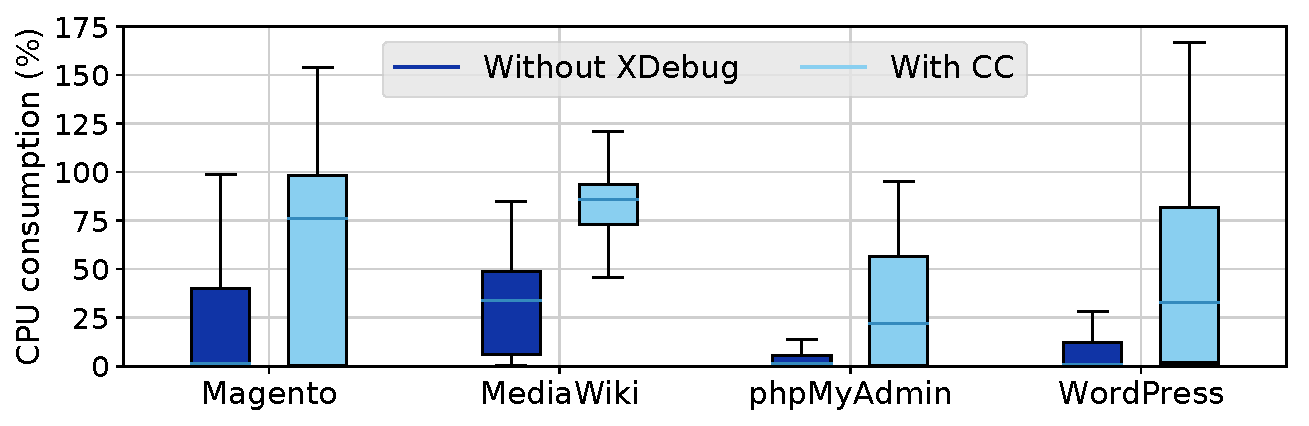
\includegraphics[width=\linewidth]{figures/lim/cpu.pdf}
  \caption{Measurement of the CPU consumption for the tested web
  applications. 100\% corresponds to the use of a single CPU core.}
  \label{fig:cpu}
\end{figure}